% Autor: Alfredo Sánchez Alberca (email:asalber@ceu.es)
\begin{tikzpicture}[every label/.style={text=color1}]
\tikzstyle{node} = [align=center, node distance=1cm]; 
\tikzstyle{arrow} = [-latex, color1, line width=12pt];

\node (population) [label=-90:Population] at (0,0) {
\includegraphics[height=2cm]{img/introduction/population.pdf}}; 
\node (sample) [label=-90:Sample] at (6,0) {\includegraphics[height=2cm]{img/introduction/sample.png}};
\node at (3.3,0) [fill=color1,single arrow,shape border rotate=0,text=white, minimum width=1.2cm]{
\ Sampling\ \phantom{}};
\end{tikzpicture} 